\documentclass{VUMIFPSbakalaurinis}
\usepackage{algorithmicx}
\usepackage{algorithm}
\usepackage{algpseudocode}
\usepackage{amsfonts}
\usepackage{amsmath}
\usepackage{bm}
\usepackage{biblatex}
\usepackage{caption}
\usepackage{color}
\usepackage{float}
\usepackage{graphicx}
\usepackage{listings}
\usepackage{subfig}
\usepackage{wrapfig}
\usepackage{enumitem}
% Global settings for enumerator.
\setitemize{noitemsep,topsep=0pt,parsep=0pt,partopsep=0pt}
\setenumerate{noitemsep,topsep=0pt,parsep=0pt,partopsep=0pt}
\setdescription{noitemsep,topsep=0pt,parsep=0pt,partopsep=0pt}

% Titulinio aprašas
\university{Vilniaus universitetas}
\faculty{Matematikos ir informatikos fakultetas}
\department{Programų sistemų katedra}
\papertype{Bakalauro darbas}
\title{Neuroninių tinklų panaudojimas testavimo proceso gerinimui}
\titleineng{Using Neural Networks to Improve the Testing Process}
\author{Ričardas Mikelionis}
% \secondauthor{Vardonis Pavardonis}   % Pridėti antrą autorių
\supervisor{asist. dr. Vytautas Valaitis}
\reviewer{partn. prof., dr. Aldas Glemža}
\date{Vilnius – \the\year}

% Nustatymai
\setmainfont{Palemonas}   % Pakeisti teksto šriftą į Palemonas (turi būti įdiegtas sistemoje)
\bibliography{bibliografija}

\begin{document}
\maketitle

%% Padėkų skyrius
% \sectionnonumnocontent{}
% \vspace{7cm}
% \begin{center}
%     Padėkos asmenims ir/ar organizacijoms
% \end{center}

\sectionnonumnocontent{Santrauka}
Glaustai aprašomas darbo turinys: pristatoma nagrinėta problema ir padarytos
išvados. Santraukos apimtis ne didesnė nei 0,5 puslapio. Santraukų gale
nurodomi darbo raktiniai žodžiai. 
% Nurodomi iki 5 svarbiausių temos raktinių žodžių (terminų).
% Vienas terminas gali susidėti iš kelių žodžių.
\raktiniaizodziai{raktinis žodis 1, raktinis žodis 2, raktinis žodis 3, raktinis žodis 4, raktinis žodis 5}   

\sectionnonumnocontent{Summary}
Santrauka anglų kalba. Santraukos apimtis ne didesnė nei 0,5 puslapio.
\keywords{keyword 1, keyword 2, keyword 3, keyword 4, keyword 5}

\tableofcontents

\sectionnonum{Įvadas}
Smarkiai augant Continuous Delivery principų populiarumui auga poreikis testuoti daugiau per trumpesnį laiko tarpą. Paprastas sprendimas šiai problemai būtų be abejo nuolat besisukantis automatinių testų paketas, tačiau automatiniais testais padengti programinį kodą 100\% praktiškai neįmanoma. 100\% padengimas įmanomas tik pagal kokią nors specifinę metriką, o vaikytis tikrojo 100\% padengtumo testais pagal kiekvieną metriką ar funkcinę sritį prilygsta šviesos geičio vaikymuisi, kuo arčiau esame tikslo tuo daugiau pastangų ir resursų reikia pasistūmėti į priekį. Todėl, žinoma, vis dar išlieka poreikis rankiniam testavimui. Norint išleisti programinės įrangos versiją kuo dažniau ištestuoti visko kiekvieną kartą neįmanoma. Taip šis problemos sprendimas iškelia dar vieną, mažesnę, problemą: kaip efektyviai pasirinkti testavimo sritis kiekvienai naujai programos laidai (angl. release). Alan M. Davis \cite{Davis:1995:PSD:203406} tegia, jog pareto principą galima pritaikyti ir programinės įrangos testavime: čia 80\% kode esančių defektų surandami 20\% viso kodo.

Tobulame pasaulyje iteracijai pasirinktos testavimo sritys ir apims tuos 20\% problematiškojo kodo. Tačiau dažnai net remiantis visa turima istorine informacija testuotojui atsakingam už testavimo sričių parinkimą yra sunku efektyviai atrinkti testavimo sritis, kuriose atliktas darbas turės didžiausią įtaką programinės įrangos kokybei.

Pagrindiniai kriteriai pagal kuriuos dabar įparstai prioritetizuojami programinės įrangos moduliai testavimui yra: paskutinis modulio testavimo laikas, kuo ilgensį laiko tarpą netestuota tuo aukštesnę pirmenybę modulis įgauna, modulio naujumas, visiškai nauji programinės įrangos moduliai privalo būti testuojami, modulio atnaujinimas, jei modulis išplėstas ar sumažintas funkcionalumo prasme jis turi aukštą pirmenybę būti testuojamas ir galiausiai praeityje defektyvūs moduliai, tai tokie moduliai kurie praeityje turėjo defektų ir šie buvo ištaisyti.

Dažnai turint mažai laiko testuoti, modulių prioritetiavimas sueikvoja nemažą dalį laiko, kurį būtų galima testuoti, taip pat dažnai tenka palikti daug aukšto prioriteto modulių nepilnai ištestuotus ar visai netestuotus. Tai didina programinės įrangos riziką būti nekokybiška. Ypač kai defektai lieka nesurasti keletą laidų (angl. release) ir po to tenka aiškintis ar defektas reiškia įvykusią regresiją ar jis visuomet egzistavo testuotame modulyje.

Tyrimui atlikti naudojama programinė įranga Weka skirta duomenų analizei bei darbui su duomenimis, Keras bei Scikit-Learn python bibliotekų paketai skirti besimokančių mašinų modeliams aprašyti.

Darbo tikslas: pateikti laiką ir pastangas taupantį testuojamų sričių atrinkimo sprendimą pasitelkiant kodo analizės metodus bei kompiuterinius neuroninius tinklus.

Siekiant sėkmingai įgyvendinti darbo tikslą bus įgyvendinti šie uždaviniai:
\begin{enumerate}
\item Išrinkti kodo metrikas darančias įtaką programinės įrangos defektyvumui
\item Palyginti efektyvumą tarp sprendimų medžio besimokančios mašinos ir neuroninio tinklo naudojant surinktus duomenis
\item Atrinkti bei atmesti duomenis turinčius mažiausią įtaką galutiniam spėjimui
\item Naudojantis mažesniu atributų kiekiu iš naujo apmokyti neuroninį tinklą ir palyginti rezultatus su pilnų duomenų rinkinių apmokyto neuroninio tinklo
\end{enumerate}

Atsižvelgiant į užduotis darbas išskirstytais skyriais bei poskyriais perteikiančiais tyrimo vykdymo eigą:
\begin{itemize}
\item 1-ame skyriuje bus apžvelgiama keletas programinės įrangos matavimo būdų stengiantis rasti ar pagrįsti ryšį su programinės įrangos defektyvumu.
\item 2-ame skyriuje programinės įrangos metrikos turinčios ryšį su programų defektyvumu apdorojomos keletu skirtingų besimokančių mašinų ir palyginami jų tikslumo rezultatai.
\item 3-iame skyriuje duomenų rinkiniams atliekami duomenų atrinkimo procesai siekiant pašalinti besimokančioms mašinoms efekto neturinčius duomenis.
\item 4-ame skyriuje pateikiami rezultatai naujų besimokančių mašinų pritaikytų dirbti su atnaujintais duomenų rinkiniais bei palyginami jų rezultatai.
\end{itemize}
 
\section{Programinio kodo sudėtingumo ir defektyvumo sąsajos}
Kiekvieną kartą renkatis testuojamas programinės įrangos vietas, žinoma, jei nėra testuojamas visas programinės įrangos funkcionalumas, reikia turėti atskaitos tašką, kuris leistų nuspręsti kurios programinės įrangos kodo vietos, ar programų paketo moduliai turi didžiausią riziką būti defektyvūs. Į šią kategoriją dažnai pakliūva seniai testuoti, nauji, atnaujinti bei anksčiau daug defektų turėję programinės įrangos moduliai. Didelė problema, su kuria vis dažniau susiduriama yra ką daryti, jei nėra laiko ištestuoti visiems šiems moduliams ir kaip tuomet pasirinkti atitinkamus progaminės įrangos modulius testavimui, kad nešvaistydami laiko padarytumėme didžiausią įmanomą įtaką programinės įrangos kokybės užtikrinimui. 

Visų pirma reikėtų sukurti detalesnę programinės įrangos metrikų sistemą nei, „naujumas“ ar „prieš tai buvusių defektų kiekis“, kuri tiesiogiai atspindėtų būsimą (ar esamą) programinės įrangos defektyvumą. O gal būt užtenka pritaikyti egzistuojančias programinio kodo metrikas randant koreliaciją su programų defektyvumu. Ir iš tiesų, būtų galima teigti, jog programinės kokybės metrikos kurias būtų įmanojma tiesiogiai susieti su programinio kodo defektyvumu egzituoja. Arčiausiai tokių metrikų yra programino kodo sudėtingumo metrikos. Be abejo yra ne vienas būdas matuoti programos kodo sudėtingumą, tačiau, šiam tyrimui pasirinktos dvi, galima būtų sakyti, populiariausios metrikos kodo sudėtingumui atvaizduotii: Maurice H. Halstead aprašytosios 1977-aisiais \cite{Halstead:1977:ESS:540137} bei Thomas J. McCabe aprašytosios 1976-aisiais \cite{McCabe:1976:CM:800253.807712}. 

Ryšys tarp kodo sudėtingumo bei defektų buvimo jame, o gal būt derėtų sakyti defektų buvimo galimybės kode, atrodytų, gana logiškas: kuo sudėtingesnis kodas, tuo sunkiau jį skaityti, kuo sunkiau kodas skaitomas tuo sunkiau jį plėsti, todėl kyla rizika defektų atsiradimui. Tokia prielaida tiriama nuo pat sudėtingumo metrikų aprašymo. Žinoma, dėl kodo sudėtingumo tiksliai defektų kiekui daromo efekto kyla nestuarimų. Atsiranda teigiančių, jog Halstead metrikos neturi jokio įrodomo ryšio su defektų buvimu, tačiau yra ir tyrimų pagrindžiančių kodo sudėtingumo bei defektų buvimo jame koreliaciją \cite{Schroeder1999APG}. Dažniausiai tyrėjai lieka šio argumento viduryje nei visiškai neigdami, nei patvirtindami šią koreliaciją. Gana dažnas sprendimas yra pamažinti metrikų kiekį ir patikrinti metrikas priklausomai nuo situacijos, taip užtikrinant, kad pasirinktosios metrikos tikrai korelioja su tyrimo metu ieškomu fenomenu, šiuo atveju kodo defektyvumu \cite{Metrics in Evaluating Software Defects:2013}.

Tokių metrikų pasirinkimas paremtas tuo, jog jų rinkimas, net atliekamas nuolat nereikalauja daug papildomo laiko, išteklių ar pastangų. Tai statinės kodo metrikos, kurias gana paprasta surinkti su kodo analizės įrankiais ir kurios sąlyginai tikliai parodo kodo defektyvumą.

Šiame dokumente aprašomame tyrime bus naudojamos visos Halstead ir McCabe metrikos kartu, bei keletas šių atributų poaibių susiaurintų tiek rankiniu būdų tiek duomenų analizės įrankiais.

\subsection{McCabe sudėtingumo metrikos}
1976-aisiais Thomas J, McCabe išleido tyrimą kuriame pasiūlė naują programinės įrangos kodo sudėtingumo matavimo būdą, pavadintą Ciklomatiniu sudėtingumu (angl. Cyclomatic Complexity). Šis matavimo vienetas kiekybiškai matuoja nepriklausomų kelių per kodo elementus kiekį.

Ciklomatnis sudėtingumas apibrėžiamas, kaip kodo vykdyme egzistuojančių tiesiškai nepriklausomų kelių kiekis. Pavyzdžiui jei kode nėra jokių eiliškumo kontrolės sakinių (angl. Control flow statements), kaip sąlygninai „if“ sakiniai, tuomet kodo ciklomatinis sudėtingumas būtų 1. Su vienu „if“ sąlyginiu sakiniu, po kurio įvykdymo galimi du keliai: jei grąžinta „TRUE“ bei jei grąžinta „FALSE“, kodo ciklomatinis sudėtingumas būtų 2. Du vieną sąlygą turintys „if“ sakiniai ar vienas toks sakinys su dviem salygomis sudarytų grafą kurio ciklomatinis sudėtingmas būtų lygus 3 ir t.t. \cite{McCabe:1976:CM:800253.807712}

Ciklomatinis sudėtingumas skaičiuojamas naudojant orientuotą grafą, kuris vaizduoją programos kodą. Tokiu atveju grafo viršūnės atspindi komandų, kurios vykdomos kartu, grupes, o kraštinė su kryptimi sujungia dvi viršūnes jei jos gali būti vykdomos viena po kitos. Tokį ciklomatinio sudėtingumo skaičiavimo metodą galima taikyti ir aukštesnės abstrakcijos progaminio kodo vienetams kaip funkcijos, metodai, klasės ar kt.

Matematiškai ciklomatinis sudėtingumas M apskaičiuojamas formule \(M = E - N + 2P\). Kur šios metrikos atvaizduojamos taip:
\begin{description}  
\item E = grafo kraštinių kiekis,
\item N = grafo viršūnių kiekis,
\item P = apjungtų komponentų kiekis.
\end{description} 
Dar cikomatinis sudėtingumas skaičiuojamas ir formule \(M = E - N + P\). Šiuo atveju kodas vaizduojamas grafu kurio pradinio ir paskutinio modulio grafo viršūnės yra sujungtos, taip sudarant stipriai apjungtą grafą, ir kodo ciklomatinis sudėtingumas prilygsta grafo ciklomatiniam skaičiui.

Pavyzdžiui, turint programą, kaip pavaizduota pav. \ref{img:Cyclomatic_graph_1} kurios veikimas prasideda nuo modulio atvaizduoto raudona viršūne, o kodo vykdymas pabaigiamas įvykdžius mėlyna viršūne atvaizduotą kodą galime panaudoti McCabe formulę ir apskaičiuoti kodo ciklomatinį sudėtingumą. Toks grafas sudarytas iš devynių kraštinių bei aštuonių viršūnių, kurie kartu sudaro vieną apjungtąjį komponentą, tuomet tokios programos ciklomatinis sudėtingumas būtų \(9 - 8 + 2 * 1 = 3\).

\begin{figure}[H]
    \centering
    \includegraphics[scale=0.6]{img/Cyclomatic_graph_1}
    \caption{Programinio kodo atvaizdavimas grafu}
    \label{img:Cyclomatic_graph_1}
\end{figure}



\subsection{Halstead sudėtingumo metrikos}
1977-aisiais Maurice H. Halstead, knygoje „Elements of Software science“ pateikė kodo sudėtingumo metrikas kaip būdą programinės įrangos kūrimą paversti empiriniu mokslu. Halstead metrikos tiesiogiai priklauso nuo to, kaip kodas parašytas ir yra skaičiuojamos statiškai, pagal operatorius bei operandus. Pasak M. H. Halstead kompiuterinė programa yra tiesiog algoritmo realizacija, sudaryta iš operatorių bei operandų sekos.\cite{Halstead:1977:ESS:540137}

Halstead metrikos paremtos šiais matavimo vienetais:
\begin{description}  
\item\(n_1\) - unikalių operatorių kiekis,
\item\(n_2\) - unikalių operandų kiekis,
\item\(N_1\) - visų operatorių kiekis,
\item\(N_2\) - visų operandų kiekis.
\end{description} 
Iš šių matų šskaičiuojami šios metrikos:
\begin{description}  
\item\(n =  n_1 + n_2\) - Programos žodynas,
\item\(N = N_1 + N_2\) - programos dydis,
\item\(V = N * log_2n\) - programos apimtis,
\item\(D = \frac{n_1}{2} * \frac{N_1}{n_2}\) - programos sudėtingumas,
\item\(E = D * V\) - pastangos.
\end{description} 
Čia programos sudėtingumas reiškia sudėtingumą skaitant ar rašant tolesnį kodą pvz. atliekant kodo peržiūrą.

Halstead metrikos dažnai kritikuojamas dėl neapibrėžto operatorių bei operandų nustatymo būdų, dažnai kritikos susilaukia ir tai, jog matuojamas tekstu pagrįstas sudėtingumas, t.y. kaip sunku skaityti kodą, o ne sudėtingumas pagrįstas kodo struktūra ar logika.

\section{Sudėtingumo metrikų panaudojimas aprašant programinės įrangos defektyvumą nuspėjančią besimokančią mašiną}

Turint aiškiai apibrėžtas metrikas programinės įrangos kodui apibūdinti galima būtų vesti žurnalą kiekvienam programinės įrangos moduliui ir kiekvieną kartą renkantis programinės įrangos sritis, kurias reikia testuoti, palyginti esamos kodo laidos (angl. release) metrikas su žurnale esančiomis taip nuspriandžiant ar išanalizuotą sriti reikia testuoti dabar ar sričiai priskirti žemesnę pirmenybę. Tačiau toks procesas atliekamas rankiniu būdu ne tik, kad ne taupo laiko, tačiau ir prideda papildomų rūpesčių testuotojams sprendžiantiems testų prioritetus. Iš to turime problemą kuri dažnai sprendžiama automatizuojant ir viską aprašant besimokančia mašina. Šiame tyrime bus naudojamos dviejų tipų besimokančios mašinos: Sprendimų medžio spėjamasis modelis bei daugiasluoksniu perceptronu aprašytą neuroninį tinklą.

Apmokyti šias besimokančiasias mašinas bus naudojama kombinacija atributų gautų kodo statinės analizės metu, ir Halstead bei McCabe metrikų apskaičiuotų naudojant statinės analizės metu surinktus duomenis. Iš viso duomenų lentelė kuri bus pateikta besimokančiai mašinai susidės iš 22 stulpelių: 21 atributo bei 1 stulpelio reiškiančio defektų egzistavimą. Reikšmės žymimos taip:
\begin{description} 
\item loc - Skaitinė reikšmė. McCabe eilučių kode kiekis.
\item v(g) - Skaitinė reikšmė. McCabe ciklomatinis sudėtingumas.
\item ev(g) - Skaitinė reikšmė. McCabe esminis sudėtingumas.
\item iv(g) - Skaitinė reikšmė. McCabe dizaino sudėtingumas.
\item n - Skaitinė reikšmė. Halstead visų operatoriu bei operandų suma (programos dydis).
\item v - Skaitinė reikšmė. Halstead programos apimtis.
\item l - Skaitinė reikšmė. Halstead programos ilgis.
\item d - Skaitinė reikšmė Halstead sudėtingumas.
\item i - Skaitinė reikšmė. Halstead protingo turinio metrika.
\item e - Skaitinė reikšmė. Halstead pastangos.
\item b - Skaitinė reikšmė. Halstead defektų kiekio spėjimas.
\item t - Skaitinė reikšmė. Halstead laiko suprogramuoti metrika.
\item lOCode - Skaitinė reikšmė. Halstead kodo eilučių kiekis.
\item lOComment - Skaitinė reikšmė. Halstead komentarų eilučių kiekis.
\item lOBlank - Skaitinė reikšmė. Halstead tuščių eilučių kiekis.
\item lOCodeAndComment - Skaitinė reikšmė. Komentarų bei kodo eilučių kiekių sumą.
\item uniq\_Op - Skaitinė reikšmė. Unikalių operatorių kiekis.
\item uniq\_Opnd - Skaitinė reikšmė. Unikalių operandų kiekis.
\item total\_Op - Skaitinė reikšmė. Visų operatorių kiekis.
\item total\_Opnd - Skaitinė reikšmė. Visų operandų kiekis.
\item branchCount - Skaitinė reikšmė. Grafu atvaizduojamo kodo kelių kiekis.
\item defects - Binarinė reikšmė. True arba False.
\end{description} 

Tyrimo tikslui pasiekti buvo nuspręsta panaudoti keletą jau surinktų duomenų rinkinių. Siekiant surinkti pakankamą kiekį prasmingų duomenų (500-1000 skirtingų testuotų programinės įrangos versijų (angl. build)) šio tyrimo kontekste užimtų per daug laiko. Tyrime bus naudojami  „CM1“ bei „PC1“ duomenų rinkiniai iš  „Promise“ duomeų rinkinių duomenų bazės \cite{Sayyad-Shirabad+Menzies:2005}. Tiek „CM1“, tiek „PC1“ pateikti NASA ir sudaryti jų 2004-aisiais vykdytos „NASA Metrics Data Program“ progamos, skirtos kurti defektus nuspėjančią programinę įrangą, metu.

PC1 duomenų rinkinys sudarytas iš 1109 duomenų eilučių, surinktų iš kodo parašyto C programavimo kalba. Programinė įranga iš kurios surinkti šie duomenys skirta orbitoje skraidančiam palydovui kontroliuoti. Duomenų rinkinys pasidalina į 6.94\% duomenų eilučių kurios atspindi atvejį, kai užfiksuotas vienas ar daugiau defektų bei 93.06\% duomenų eilučių atspindinčių, kai nebuvo užfiksuota defektų.

CM1 duomenų rinkinys sudarytas iš 498 duomenų eilučių, surinktų iš kodo parašyto C programavimo kalba. Programinė įranga iš kurios surinkti šie duomenys yra pagalbinė įranga vienam iš NASA erdvėlaivių. Duomenų rinkinys pasidalina į 90.16\% duomenų eilučių kurios atspindi atvejį, kai užfiksuotas vienas ar daugiau defektų bei 9.83\% duomenų eilučių atspindinčių, kai nebuvo užfiksuota defektų.

\subsection{Sprendimų medžio metodu paremta besimokanti mašina}
Pirmasis prediktyvusis modelis paremtas sprendimų medžio klasifikatoriumi. Toks modelis yra laisvai suprantamas ir skaitomas net ir paprastam žmogui. Vienas tokių modelių sugeneruotas naudojant PC1 duomenų rinkinio poaibį pavaizduotas pav. \ref{img:tree} pirmame priede. 

Su tradiciniais duomenų rinkiniais sprendimų medis turi nemažai privalumų. Sprendimo medžiai yra lengvai suprantami, net daug techninių žinių neturintiems žmonėms ir pateikus sprendimų medį grafiškai pačiam galima pereiti per viršūnes tikrinant duomenų rinkinio eilutės grąžinamą rezultatą. Taip pat palyginus su kitais prediktyviaisiais modeliais sprendimo medžiai reikalauja salyginai nedidelio kiekio duomenų pertvarkymo prieš naudojant juos šiame modelyje. Iki tam tikro laipsnio smarkiai išsiskiriančios reikšmės ar trūstami įrašai nedaro didelės įtakos sprendimų medžiams. Sprendimų medžiai neskiria ir gali priimti tiek skaitines tiek logines reikšmes, todėl galima naudoti didesnę įvairovę duomenų rinkinių.

Didžiausi sprendimų medžio trūkumai yra tikslumo trūkumas, kadangi tai, ginčytinai, paprasčiausias besimokančios mašinos modelis jis yra ir pats netiksliausias. Modelio paprastumas su dideliais duomenų rinkiniais gali privesti prie per sudėtingo medžio sugeneravimo, kuomet nebeatpažystami ryšiai tarp atributų bei galutinio rezultato. Tai dažnai vadinama permokymu (angl. overfitting).

Įprastai sprendimų medžio prediktyvusis modelis naudojamas salyginai paprastų duomenų rinkinių problemoms spręsti. Žemo lygio klasifikatoriams bei prediktyviesiems modeliams, kaip Iriso gėlės skirtingų rūšių klasifikavimo problema.

Šio tyrimo metu sprendimų medžio modelis ir klasifikatorius buvo aprašyti ir įgyvedinti Python kalba paraštu scriptu naudojant medžio biblioteką pateiktą Scikit-learn \cite{scikit-learn}.

Rezultatai taip pat buvo apskaičiuoti keletu scikit-learn pateiktų bibliotekų, kurių viduje jie apskaičiuojami keletu formulių:
\begin{description} 
\item \(Precision = \frac{\Sigma Tikras pozityvas}{\Sigma Tikras pozityvas + \Sigma Netikras pozityvas}\)
\item \(Accuracy = \frac{\Sigma Tikras pozityvas + \Sigma Tikras negatyvas}{\Sigma Tikras pozityvas  + \Sigma Tikras nNegatyvas + \Sigma Netikras pozityvas + \Sigma Netikas negatyvas}\)
\item \(Recall = \frac{\Sigma Tikras pozityvas}{\Sigma Tikras pozityvas + \Sigma Netikras negatyvas}\)
\end{description}
kur „Tikrasis pozityvas“ yra teisingai nustatyta pozityvi reikšmė, „Tikrasis negatyvas“ yra teisingai nustatyta negatyvi reikšmė, „Netikras pozityvas“ yra klaidingai nustatyta pozityvi reikšmė, o „Netikras negatyvas“ yra neteisingai nustatyta negatyvi reiškmė.

Besimokančių mašinų kontekste Accuracy reiškia kiek procentaliai iš visų spėtų reikšmių buvo atspėta teisinga reikšmė. Precision parodo kiek iš atspėtų teigiamų reikšmių yra tikrų pozityvų, t.y. teisingai nuspėtų teigiamių reikšmių. O Recall parodo kiek tarp iš viso buvusių teigiamų reikšmių jų buvo atspėta.

\begin{table}[H]\footnotesize
\centering
\caption{Sprendimų medžio mašinos rezultatai}
\label{tab:Tree_result}
\begin{tabular}{lllll}
\cline{1-4}
\multicolumn{1}{|l}{Duomenų rinkinys} & accuracy & precision & \multicolumn{1}{l|}{recall} &  \\ \cline{1-4}
\multicolumn{1}{|l}{PC1}              & 90\%   & 30\%     & \multicolumn{1}{l|}{35\%} &  \\
\multicolumn{1}{|l}{CM1}              & 84\%    & 13.3\%     & \multicolumn{1}{l|}{21\%}  &  \\ \cline{1-4}
                                      &          &           &                             & 
\end{tabular}
\end{table}

Lentelė \ref{tab:Tree_result} atvaizduoja accuracy, percision bei recall reikšmes gautas iš sprendimų medžiu paremto modelio. Modeliui apmokyti ir testuoti abiem atvejais buvo panaudotas visas duomenų rinkinys su 21 atributu, kur 50\% atsitiktinai atrinktų reikšmių buvo panaudotos, kaip mokomieji duomenys, o kiti 50\%, kaip testiniai.

Sprenimo medžiu paremtas prediktyvus modelis daug nežada. Su CM1 duomenų rinkiniu turime didelį, bet toli gražu ne patį geriausią accuracy, o visais atvejais tiek precision tiek recall reikšmės nesiekė 50\%. Galima būtų kelti hipotezę, jog didžiausią problemą sukelia duomenų rinkiniai turintys 21 atributą ir labai nelygų duomenų pasiskirstymą, kodėl čia išvydome „permokymo“ reiškinį. Tačiau pirmiausia reikėtų patikrinti ar su tokiais pat, ne modifikuotais, duomenimis galima gauti gerensius rezultatus naudojant kitokį klasifikatorių.

\subsection{Daugiasluoksnis perceptronas}
Antrasis prediktyvusis modelis tyrimo metu buvo aprašytas Daugiasluoksio perceptrono klasifikatoriumi. Siekiant didelio efektyvumo šiame modelyje pridėti du sluoksniai su vis mažesniu kiekiu neuronų, taip bemokant modelį priverčiant jį atskirti svarbiausias reikšmes darančias didžiausią įtaką galutiniam rezultatui. Taip pat po kiekvieno iš paslėptųjų sluoksnių įterptas išmetimo sluoksnis, kuris apmažina praeitame sluoksnyje sukurtų ryšių kiekį taip mažinant tinklo permokymo galimybę \cite{JMLR:v15:srivastava14a}. Tokiu atveju tinklas tampa panašenis į tokį, vaizduojamą dešinėje pav. \ref{img:dropout}

\begin{figure}[H]
    \centering
    \includegraphics[scale=0.5]{img/dropout}
    \caption{„Dropout“ sluoksnių efektas daugiasluoksniam perceptronui.}
    \label{img:dropout}
\end{figure}

Toliau šiame tyrime naudojamas daugiasluoksnio perceptrono modelis atrodys taip, kaip vaizduojama pav. \ref{img:model}, kur įvesties (angl. input) sluoksnyje turime 21 atributą, kaip ir duomenų rinkinyje, toliau du užslėptus sluoksnius, su trečdaliu mažiau įvesčių siekiant sukurti glaudesnius ir prasmingenius ryšius tarp modelio viršūnių, kas kart apmažinant ryšių kiekį siekiant išvengti modelio permokymo.

\begin{figure}[H]
    \centering
    \includegraphics[scale=0.5]{img/model}
    \caption{Daugiasluoksnio perceptrono struktūra}
    \label{img:model}
\end{figure}

Daugiasluoksnis perceptronas taip pat dažnai naudojamas paprastų duomenų rinkinių, atvaizduojamų lentele, analizei. Šio tyrimo kontekste toks neuroninis tinklas tinkamiausias, nes daugeliu kitų atvejų, pavyzdžiui konvoliucinio neuroninio tinklo, kuris savo struktūra yra sudėtingesnis bei daugeliu atvejų efektyvesnis, reikėtų adaptuoti bei transformuoti duomenų rinkinį, to buvo siekiama išvengti kuo tikslesniam palyginimui su sprendimų medžio modeliu.

Daugiasluoksnis perceptronas buvo aprašytas Python programavimo kalbą pasinaudojus „Tensorflow“ paremtu python bibliotekų rinkiniu skirtu darbui su sekvenciniais neuroniniais tinklais „Keras“ \cite{chollet2015keras}. Kaip ir sprendimų medžio atveju buvo skaičiuojamos reikšmės matuojančios neuroninio tinklo accuracy, precision ir recall reikšmes.

Neuroniniam tinklui apmokymas ir testavimas vyko du kart. Vieną kartą naudojant PC1 duomenų rinkinį, kitą kartą naudojant CM1. Abiejais atvejais buvo panaudotas pilnas duomenų rinkinys su 21 atributu, kur 30\% duomenų buvo skiriama apmokyto modelio testavimui, o 70\% duomenų buvo skirta modelio apmokymui.

\begin{table}[H]\footnotesize
\centering
\caption{Daugiasluoksnio perceptrono rezultatai}
\label{tab:MLP_result}
\begin{tabular}{lllll}
\cline{1-4}
\multicolumn{1}{|l}{Duomenų rinkinys} & accuracy & precision & \multicolumn{1}{l|}{recall} &  \\ \cline{1-4}
\multicolumn{1}{|l}{PC1}              & 93.06\%   & 92.98\%     & \multicolumn{1}{l|}{92.94\%} &  \\
\multicolumn{1}{|l}{CM1}              & 90.16\%    & 89.88\%     & \multicolumn{1}{l|}{89.86\%}  &  \\ \cline{1-4}
                                      &          &           &                             & 
\end{tabular}
\end{table}

Taigi, lentelė \ref{tab:MLP_result} atvaizduoja abiejų eksperimentų su pilnų duomenų rinkiniu rezultatus, ir iš karto galime pamatyti, jog jau vien accuracy reikšmė keletu procentų aukštesnė, nei sprendimų medžio, abejais atvejais, Tačiau abi pasirinktosios metrikos naudojamos šiame tyrime turi nemažai tiesiogiai vieni kitiems proporcingų reikšmių, kurias pašalinus būtų galima dar labiau padidinti neuroninio tinklo efektyvumą sukuriant glaudesnius ryšius tarp mažesnio atributų skaičiaus.

\section{Duomenų atrinkimas}

Neatrūšiuoti duomenys skirti apmokyti neuroninius tinklus, sudaryti iš didelės įvairovės atributų, kurių tik dalis daro įtaką. Atributų atrinkimas (angl. feature selection) yra dažna praktika skirta padidinti neuroninio tinklo efektyvumą bei išvengti tinklo permokymo.

Tęsiant tyrimą bus vykdomi du skirtingi atributų atrinkimo metodai. Pradedant su pilnu duomenų rinkiniu susidedančiu iš 21 atributo rankinius būdu bus atrinkti atributai, kurie tiesiogiai susiję su kitais, t.y. jei Halstead metrikos išvedamos naudojant unikalių operandų bei operatorių kiekius, šie abu atributai bus išimami iš duomenų rinkinio, o palikti tik iš jų abiejų išvesti duomenys.

Kitas duomenų atrinkimo metodas bus atliktas automatiškai, naudojant duomenų analizės įrankį „Weka“. Išbandžius keletą atrinkimo metodų bei algoritmų bus sudaryti nauji duomenų rinkiniai - senojo poiaibiai.

\subsection{Rankiniu būdu ieškant atributų kurie yra tiesiogiai proporcingi kitiems atributams}

Duomenų atrinkimas buvo pradėtas nuo Halstead reikšmių, kurios nors ir pateikia mums empirines metrikas kodui yra išvestinės, t.y. keturios metrikos apibūdinančios operandų kiekį kode yra kombinuojamos tarpusavyje gauti kitoms todėl jos yra tiesiogiai proporcingos ir perteklinės neuroninio tinklo mokymo kontekste, todėl gali vesti permokymo link. Taip pat išimtos reikšmės tiesiogiai darančios įtaką kodo skaitomumui, tačiau neturinčios jokios esminės įtakos kodo vykdyme, kaip komentarų eilučių kiekis ar tuščių eilučių kiekis.

Taip pat išimtos visos žemesnio lygio reikšmės skirtos apskaičiuoti tiek McCabe metrikas tiek papildomai pridėtos duomenų rinkinyje. Taip paliekant 10-ies atributų duomenų rinkinį sudarytą vien iš išvestinių reikšmių, kurios buvo tiesiogiai proporcingos nuo išimtųjų, tačiau tarpusavyje tokio ryšio neturi.

Po šio duomenų atrinkimo metodo duomenų rinkinio atributai atrodo taip:
\begin{description} 
\item loc - Skaitinė reikšmė. McCabe eilučių kode kiekis.
\item v(g) - Skaitinė reikšmė. McCabe ciklomatinis sudėtingumas.
\item ev(g) - Skaitinė reikšmė. McCabe esminis sudėtingumas.
\item iv(g) - Skaitinė reikšmė. McCabe dizaino sudėtingumas.
\item v - Skaitinė reikšmė. Halstead programos apimtis.
\item d - Skaitinė reikšmė Halstead sudėtingumas.
\item i - Skaitinė reikšmė. Halstead protingo turinio metrika.
\item e - Skaitinė reikšmė. Halstead pastangos.
\item b - Skaitinė reikšmė. Halstead defektų kiekio spėjimas.
\item t - Skaitinė reikšmė. Halstead laiko suprogramuoti metrika.
\item defects - Binarinė reikšmė. True arba False.
\end{description} 


\subsection{Duomenų analizė naudojant įrankį Weka}

Weka tai darbo su dideliais duomenų rinkiniais įrankis, savyje turintis mašininio mokymosi algoritmų duomenų analizės užtuotims vykdyti. Šie algoritmai gali būti pritaikyti tiesiai duomenų rinkinius atidarius per Weka grafinę sąsają, arba iškviesti Java kodu ir apdoroti naudojantis Weka bibliotekomis.

Duomenų analizės įrankis Weka \cite{hall09:_weka_data_minin_softw} turi daug su duomenų analize susijusių paskirčių, kaip vizualus duomenų lentelių atvaizdavimas, duomenų atrinkimas ir kt. Tyrimo kontekste bus panauodoti keletas Weka viduje esančių atributų atrinkimo algoritmų, kuriuos apžvelgus bus atrinkti nauji, sumažinti, duomenų rinkinai.

Iš leidžiamų pasirinkti atributų įvertinimo algoritmų šiam tyrimui tinkamiausi du: „CorrelationAttributeEval“ algoritmas kiekvieną reiškmę imantis kaip „pagrindinę“ ir lygindamas ją su kitomis grąžina koreliacijos tarp tos reikšmės bei galutinio reultato koeficientą, bei „InfoGainAttribute“ algoritmas palygindamas viso duomenų rinkinio atributų reikšmes grąžina kiekvienio atributo koeficientą reiškiantį informacijos tame atribute svarbą.

Panaudojus abu algoritmus buvo gauti tokie rezultatai:

\begin{table}[H]
\centering
\caption{Duomenų rinkinių analizės įrankiu Weka rezultatai I}
\label{tab:weka_1}
\begin{tabular}{lllllllll}
\hline
\multicolumn{1}{|l}{}                         & loc    & v(g)   & ev(g) & iv(g)  & n      & v      & l      & \multicolumn{1}{l|}{d}      \\ \hline
\multicolumn{1}{|l}{CorrelationAttributeEval} & 0.2465 & 0.1668 & 0.105 & 0.2026 & 0.214  & 0.2066 & 0.1326 & \multicolumn{1}{l|}{0.1682} \\
\multicolumn{1}{|l}{InfoGainEval}             & 0.0457 & 0.0274 & 0     & 0.0431 & 0.0426 & 0.0452 & 0.0291 & \multicolumn{1}{l|}{0.0306} \\ \hline                     
\end{tabular}
\end{table}

\begin{table}[H]
\centering
\caption{Duomenų rinkinių analizės įrankiu Weka rezultatai II}
\label{tab:weka_2}
\begin{tabular}{|llllllll|}
\hline
i & e & b & t & lOCode & lOComment & lOBlank & locCodeAndComment \\ \hline
0.2678 & 0.0978 & 0.2152 & 0.0978 & 0.063 & 0.3016 & 0.1735 & 0.0475 \\
0.0461 & 0.0391 & 0.0493 & 0.0391 & 0.02 & 0.0559 & 0.0398 & 0 \\ \hline
\end{tabular}
\end{table}

\begin{table}[H]
\centering
\caption{Duomenų rinkinių analizės įrankiu Weka rezultatai III}
\label{tab:weka_2}
\begin{tabular}{|lllll|}
\hline
uniq\_op & uniq\_opnd & total\_op & total\_opnd & branchCount \\ \hline
0.2493   & 0.2616     & 0.2141    & 0.212       & 0.1697      \\
0.0493   & 0.0499     & 0.0432    & 0.0362      & 0.0281      \\ \hline
\end{tabular}
\end{table}
Koreliacijos algoritmui renkantis reikšmes iki 0.2, o informacijos svarbos algoritmui iki 0.04 galima atrinkti ir palyginti reikšmes. Abejais atvejais gaunamas gana panašus duomenų rinkinys. Kuriuos apjungus gaunami 10 svarbiausių atributų.

Galutiniai duomenų rinkiniai bus sudaryti iš viso iš 11 stulpelių, kur paskutiniame saugomi rezultatai, o kti 10 yra pradinio duomenų rinkinio poaibis ir atrodo taip:
\begin{description} 
\item loc - Skaitinė reikšmė. McCabe eilučių kode kiekis.
\item iv(g) - Skaitinė reikšmė. McCabe dizaino sudėtingumas.
\item n - Skaitinė reikšmė. Halstead visų operatoriu bei operandų suma (programos dydis).
\item v - Skaitinė reikšmė. Halstead programos apimtis.
\item i - Skaitinė reikšmė. Halstead protingo turinio metrika.
\item b - Skaitinė reikšmė. Halstead defektų kiekio spėjimas.
\item lOComment - Skaitinė reikšmė. Halstead komentarų eilučių kiekis.
\item uniq\_Op - Skaitinė reikšmė. Unikalių operatorių kiekis.
\item uniq\_Opnd - Skaitinė reikšmė. Unikalių operandų kiekis.
\item total\_Op - Skaitinė reikšmė. Visų operatorių kiekis.
\item defects - Binarinė reikšmė. True arba False.
\end{description}

Žinoma tokia analizė nėra visiškai tiksli ir smarkiai priklauso no to koks bus pasirinktas analizės algoritmas ir kaip stuktūrizuoti bei pasiskirstę duomenys. Čia kaip matome didelę svarbą vis tiek turi eilučių, komentarų skaičiai, kurios rankiniu būdu atrenkant atributus buvo pašalintos. Šių duomenų kontekste šios reikšmės turi didelę svarbą ir padės pagerinti neuroninio tinklo rezultatus, tačiau realybėje tarp jų ir kodo defektyvumo nėra jokio glaudaus ryšio, todėl geriausia būtų naudoti šių dviejų technikų kombinaciją ir atrinkti reikšmes rankiniu būdu jas dar išanalizuoti automatiškai arba atvirkščiai.

\section{Neuroninio tinklo efektyvumo gerinimas naudojant atrinktus duomenis}

Atlikti du eksperimentai su dviemis skirtingomis besimokančiomis mašinomis, viena paremta sprendimų medžiu, o kita paremta daugiasluoksnio percetrono modeliu atvaizduotu neuroniniu tinklu. Gavus rezultatus pastebėta, jog su pilnu duomenų rinkinu sprendimų medžio mašinoje įvyksta persimokymas, o daugiasluoksnio perceptrono rezultatai, nors ir geresni, tačiau ne visai tenkina, nes egzistuoja 10\% tikimybė, jog duomenys bus indentifikuoti klaidingai.

Rezultatams gerinti priimtas sprendimas atlikti atributų išrinkimą dviem būdais. Pirmasis būdas buvo skirtas išrinkti duomenis kurie tarpusavyje neturi koreliacijos ir yra visiškai individualios reikšmės palyginus su kitais atributais. Kadangi duomenų rinkiniai sudaryti pagal McCabe ir Halstead metrikas išimti pradiniai atributai iš kurių išvestos reikšmės, taip pašalinant beveik puse visų buvusių atributų tokių kaip unikalių operandų kiekis ar kodo eilučių kiekis. Antrasis būdas buvo įvykdytas automatiškai, duomenų rinkinį įkėlus į duomenų analizės programą ir pasirinkus analizės algoritmą, kurio rezultatas svarbos reikšmės kiekvienam iš atributų. Taip pasirenkant apytiksliai puse vsų buvusių atributų.

Iš viso buvo gauti keturis naujus duomenų rinkinus, kuriuos dėl aiškumo pavadinkime PC1\_R bei CM1\_R bei PC1\_A bei CM1\_A. Čia R reiškia, jog duomenų rinkiniai buvo analizuoti rankiniu metodu, o A reiškia, jog duomenų rinkinys buvo sugeneruotas automatiškai atrinkus bei atmetus neefektyvius ir įtakos nedarančius atributus.

Tęsiant tyrimą nebenaudosime sprendimų medžio metodo, nes vien su mažiau efektyviu, pertekliniu, duomenų rinkiniu neuroninis tinklas ne tik, kad nebuvo permokytas, tačiau ir apskritai grąžino labai gerus rezultatus. Tolesnis eksperimentas bus skirtas pagerinti jau egzistuojantį neuroninio tinklo efektyvumą, taip sumažinant riziką, jog programinės įrangos versija bus neteisingai įvertinta, kaip defektyvi ir įtraukta į testavimo ciklą.

Tiesiogiai daugiasluoksnio perceptrono tinklo modeliui pritaikyti naujų duomenų rinkinių negalima. Eksperimentui su pilnu duomenų rinkiniu sukurtas daugiasluoksnis perceptronas priima tik pilną duomenų rinkinį. t.y. duomenų eilutes sudarytas iš 21 atributo. Tokiu atveju reikia atnaujinti visą modelį.

Eksperimento kontekste, norint palyginti dvi reikšmes, jos turėtu turėti tą patį pradą, t.y. būti sugeneruotos to paties modelio. Šiuo atveju modelį reikia keisti, tačiau tik pirmąjį, įvesties, sluoksnį. Pakeitus šį sluoksnį ir pritaikius naujiesiems duomenų rinkiniams eksperimentas bus vykdomas su modeliu vaizduojamu pav. \ref{img:model_adj} esančiame priede nr. 2.

Didžiausia šio modelio problema kurią realiame gyvenime galima būtų ištaisyti, tačiau tyrimo kontekste reikia palikti modelyje esantį išsiplėtimą iš 10-ies į 14-a reikšmių tarp įvesties ir pirmojo paslėpto sluoknsių. Siekiant dar geresnio modelio efektyvumo antrajame sluoksnyje galima būtų sumažinti įvesčių kiekį iki 10 ar mažiau, tačiau tokiu atveju tai būtų jau visiškai kitoks modelis, ir rezultatų palyginimas tarp 21 atributo modelio bei modelio skirto 10 atributų būtų neteisingas.

Pirma atnaujintas modelis buvo apmokytas ir ištestuotas naudojant duomenų rinkinius atrinktus rankiniu būdu, t.y. PC1\_R bei CM1\_R. Kaip ir su pilnu duomenų rinkiniu tas pat duomenų rinkinys skaidomas į dvi dalis: vieną skirtą apmokyti modelį, sudarančią 70\% viso duomenų rinkinio, o kitą - jam testuoti sudarančio 30\% viso duomenų rinkinio.

\begin{table}[H]\footnotesize
\centering
\caption{Daugiasluoksnio perceptrono rezultatai, naudojant rankiniu būdu atrinktus atributus}
\label{tab:MLP_result_1}
\begin{tabular}{lllll}
\cline{1-4}
\multicolumn{1}{|l}{Duomenų rinkinys} & accuracy & precision & \multicolumn{1}{l|}{recall} &  \\ \cline{1-4}
\multicolumn{1}{|l}{PC1\_R}              & 93.54\%   &93.32\%     & \multicolumn{1}{l|}{93.27\%} &  \\
\multicolumn{1}{|l}{CM1\_R}              & 90.45\%    & 90.39\%     & \multicolumn{1}{l|}{90.28\%}  &  \\ \cline{1-4}
\end{tabular}
\end{table}

Eksperimento rezultatai vaizduojami pav. \ref{tab:MLP_result_1}, kaip ir tikėtasi yra geresni, nei naudojant pilną duomenų rinkinį. Tačiau tikslumo pagerėjimas nėra akivaizdus ir siekia vos mažą dalelytę, galima sakyti rezultatai bene tokie pat, kaip pirmo eksperimento metu, kaip pavaizduoti pav. \ref{tab:MLP_result}.

Toliau kartojamas ekperimentas su kitais dviem duomenų rinkiniais PC1\_A bei CM1\_A. Čia taip pat duomenys dalijami į dvi dalis, 70\% apimties poaibį skirtą modelio apmokymui bei 30\% poaibį skirtą modelio testavimui.

\begin{table}[H]\footnotesize
\centering
\caption{Daugiasluoksnio perceptrono rezultatai, naudojant atributus atrinktus automatiškai Weka programa}
\label{tab:MLP_result_2}
\begin{tabular}{lllll}
\cline{1-4}
\multicolumn{1}{|l}{Duomenų rinkinys} & accuracy & precision & \multicolumn{1}{l|}{recall} &  \\ \cline{1-4}
\multicolumn{1}{|l}{PC1\_A}              & 94.02\%   & 93.86\%     & \multicolumn{1}{l|}{93.79\%} &  \\
\multicolumn{1}{|l}{CM1\_A}              & 91.05\%    & 90.89\%     & \multicolumn{1}{l|}{90.78\%}  &  \\ \cline{1-4}
\end{tabular}
\end{table}

Antrojo eksperimento su atrinktų atributų duomenų rinkiniais rezultatai dar geresni, nei rankiniu būdu atrinktų duomenų rinkinių. Tačiau vėl gi nėra ekstremalaus pokyčio palyginus su pav. \ref{tab:MLB_result}. Galima drąsiai teigti, jog atributų išrinkimas, priklausomai nuo atrinkimui naudojamo metodo, padidins neuroninio modelio tikslumą atspėjant programinės įrangos defektus. Tačiau šių duomenų rinkinių kontekste dėl keleto dešimtųjų procento, kurių nebūtų galima pavadinti smarkiu pagerėjimu, investuoti daugiau laiko ar resursų nebūtų verta.

\sectionnonum{Rezultatai ir išvados}


1.

2.

3.

4.



\printbibliography[heading=bibintoc]  % Šaltinių sąraše nurodoma panaudota
% literatūra, kitokie šaltiniai. Abėcėlės tvarka išdėstomi darbe panaudotų
% (cituotų, perfrazuotų ar bent paminėtų) mokslo leidinių, kitokių publikacijų
% bibliografiniai aprašai. Šaltinių sąrašas spausdinamas iš naujo puslapio.
% Aprašai pateikiami netransliteruoti. Šaltinių sąraše negali būti tokių
% šaltinių, kurie nebuvo paminėti tekste. Šaltinių sąraše rekomenduojame
% necituoti savo kursinio darbo, nes tai nėra oficialus literatūros šaltinis.
% Jei tokių nuorodų reikia, pateikti jas tekste.

% \sectionnonum{Sąvokų apibrėžimai}
\sectionnonum{Santrumpos}
Sąvokų apibrėžimai ir santrumpų sąrašas sudaromas tada, kai darbo tekste
vartojami specialūs paaiškinimo reikalaujantys terminai ir rečiau sutinkamos
santrumpos.

\appendix  % Priedai
% Prieduose gali būti pateikiama pagalbinė, ypač darbo autoriaus savarankiškai
% parengta, medžiaga. Savarankiški priedai gali būti pateikiami ir
% kompaktiniame diske. Priedai taip pat numeruojami ir vadinami. Darbo tekstas
% su priedais susiejamas nuorodomis.

\section{Sprendimų medžio besimokanti mašina}
\begin{figure}[H]
    \centering
    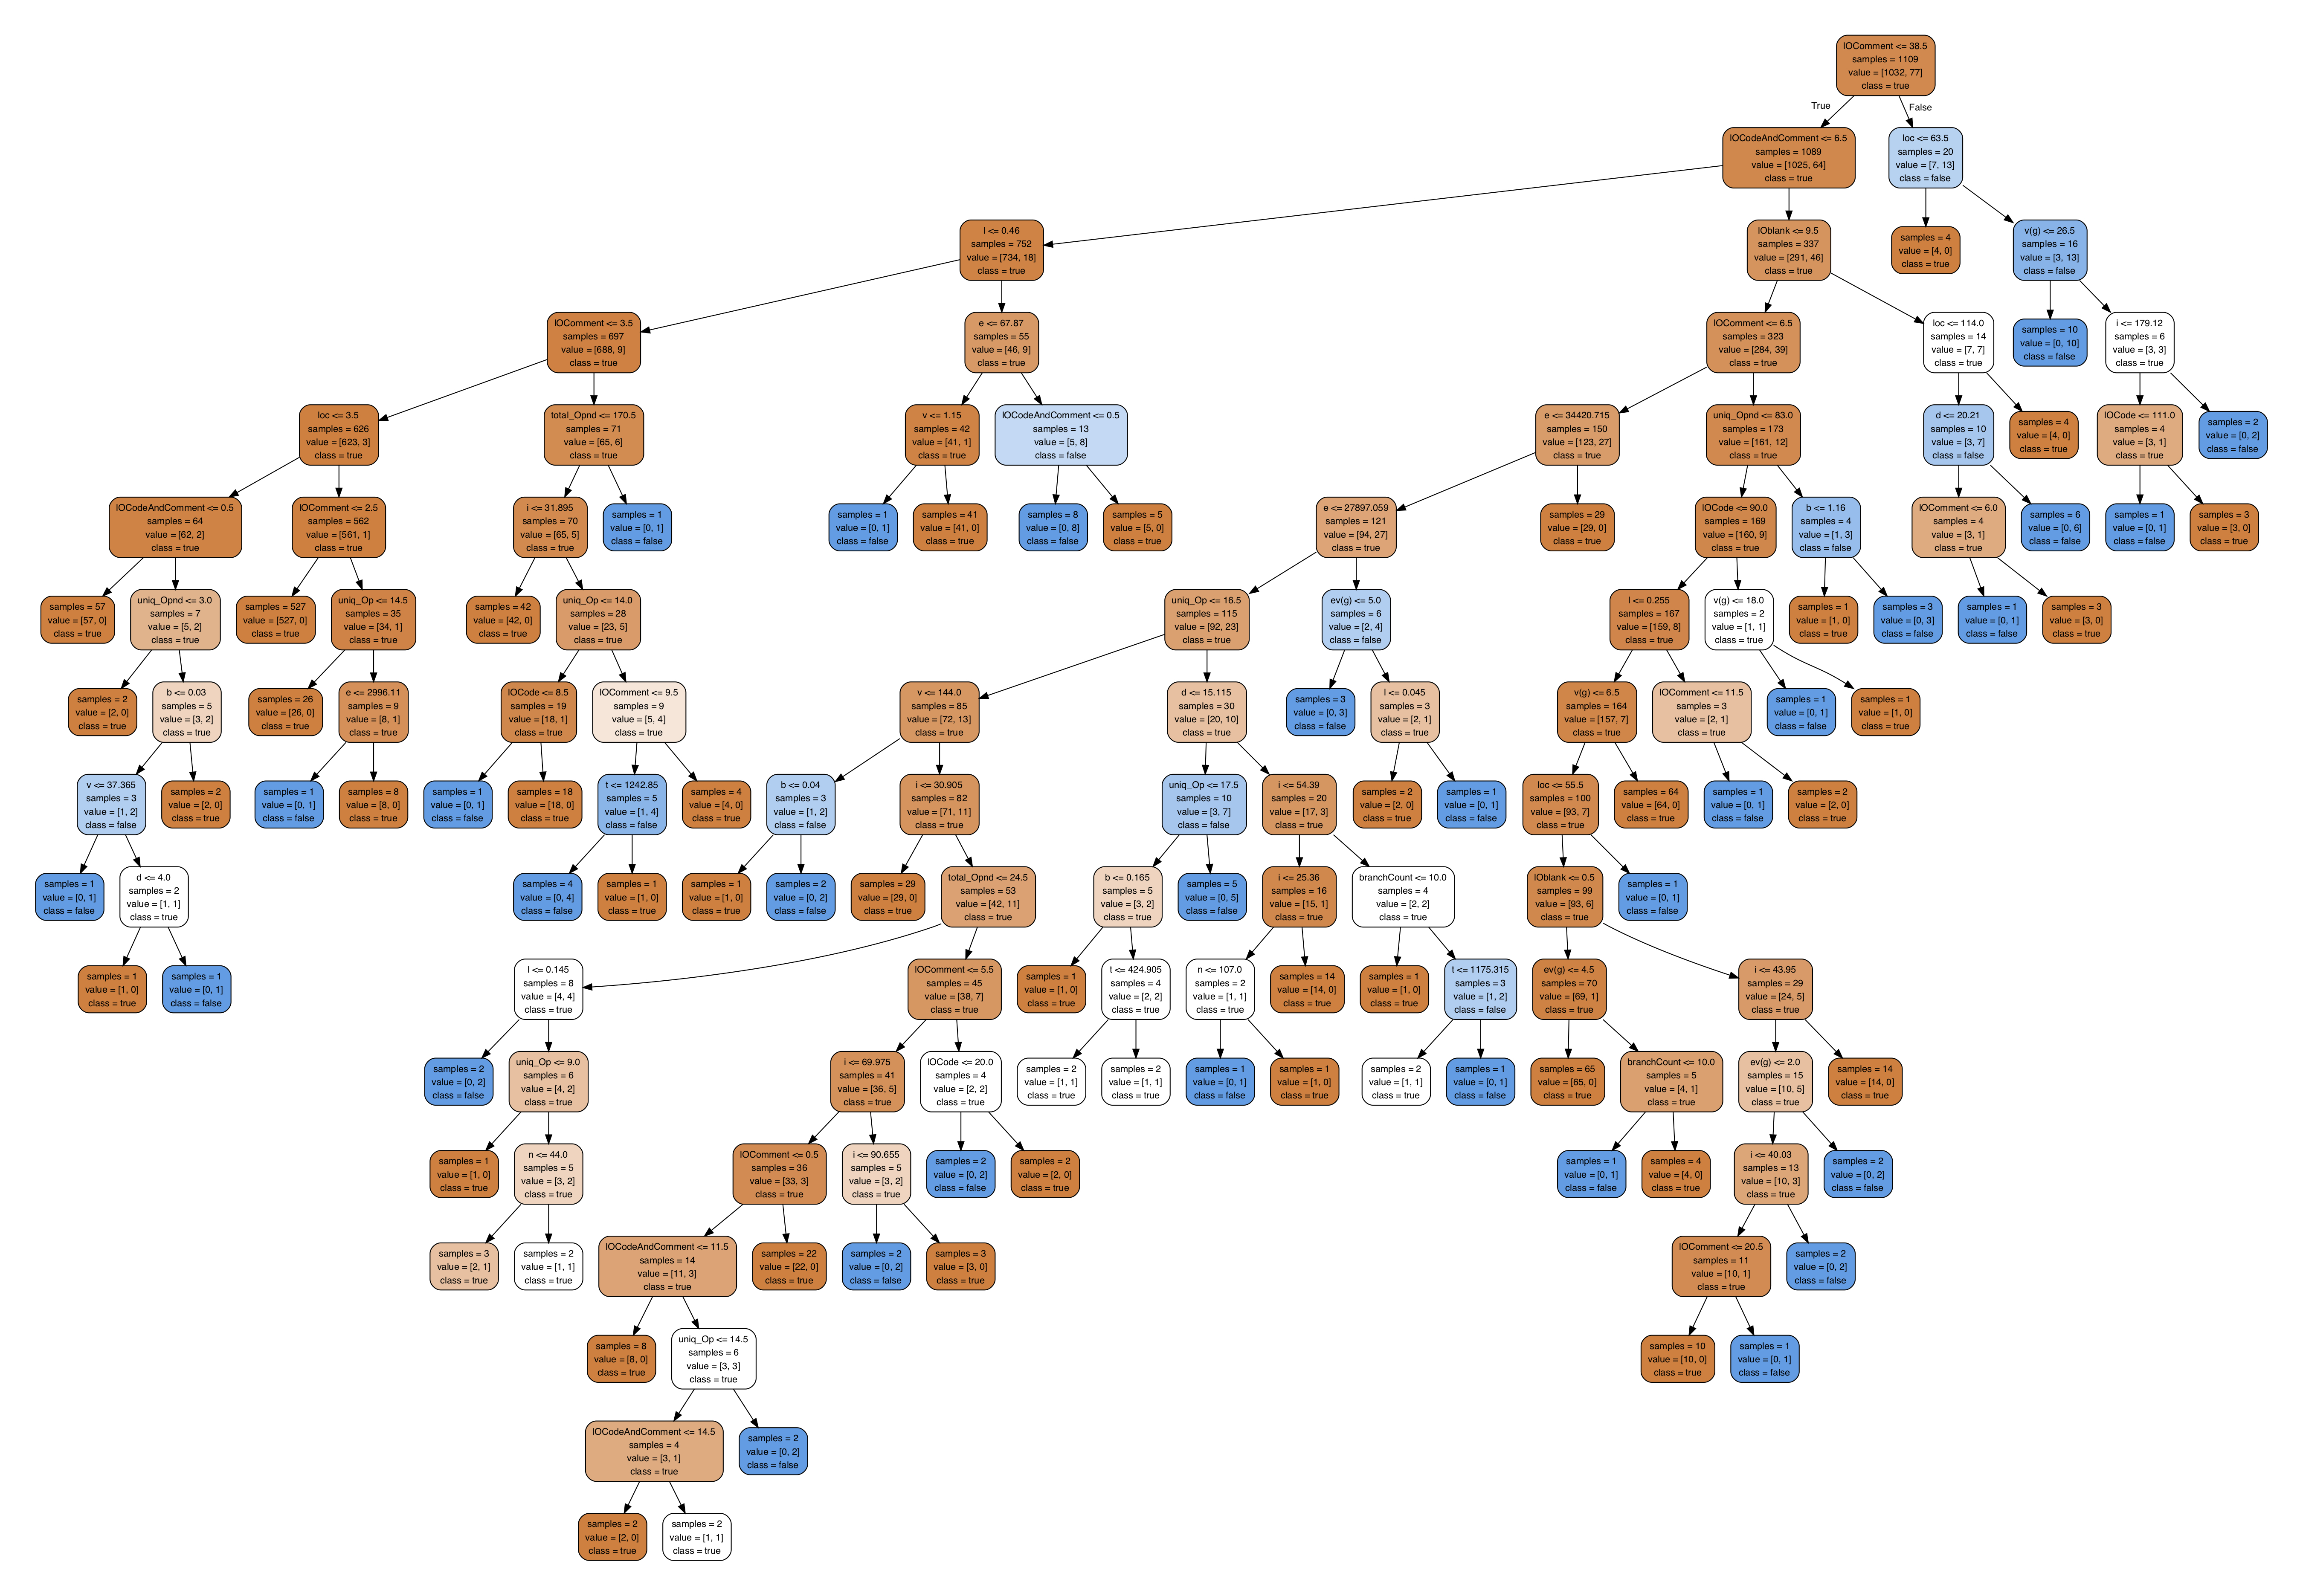
\includegraphics[scale=0.24, angle=90]{img/tree}
    \caption{Sprendimų medžio tipo besimokanti mašina sudaryta naudojant PC1 duomenų rinkinio poaibį}
    \label{img:tree}
\end{figure}


\section{Atrinktiems rezultatams pritaikyto daugiasluoksnio perceptrono struktūra}
\begin{figure}[H]
    \centering
    \includegraphics[scale=0.9]{img/model_adjusted}
    \caption{Daugiasluoksnio perceptrono struktūra atnaujinta atrinktiems atributams}
    \label{img:model_adj}
\end{figure}

\end{document}
